\documentclass[11pt]{article}

\usepackage[margin=1.1in]{geometry}
\usepackage{amsmath}
\usepackage{booktabs}
\usepackage{microtype}
\usepackage{tikz}
\usepackage[colorlinks=true,allcolors=blue]{hyperref}

\title{\textbf{Non-Normal Performance Distributions in Rating Systems}\\[0.4em]
\large with an application to seventy years of Formula 1}
\author{Peter Cotton}
\date{\today}

\begin{document}
\maketitle

\begin{abstract}
\noindent Rating systems almost universally assume that contest performance
is ability plus normal or logistic noise. We present a setting where the
assumption is visibly false and measurably costly: Formula 1, where for
decades the most likely outcome of starting a race was not finishing it. A
lattice-based Thurstonian rater that accepts arbitrary noise densities
outperforms TrueSkill, Elo, Glicko-2 and OpenSkill over 1{,}158 races, and
replacing its normal noise with a two-component density, a Gaussian pace
term plus a separated block of slow mass representing retirement, improves
every metric. Estimating the block's mass from the trailing retirement rate
improves it further. Symmetric heavy tails and skew do not help, so the
gain is attributable to the block, not to non-normality in general.
\end{abstract}

\section{Introduction}

Nearly every rating system in use rests on the same distributional
convention. A competitor's performance in a contest is modeled as a skill
parameter plus noise, and the noise is normal (Thurstone, TrueSkill, the
Thurstone--Mosteller systems) or logistic or Gumbel (Elo, Glicko,
Bradley--Terry, Plackett--Luce). The convention is so uniform that it is
rarely stated as an assumption. This paper is about what happens when it is
false, and about how much can be gained by replacing it, in a setting where
the truth is not subtle.

That setting is Formula 1. The fraction of entrants failing to finish, by
decade:

\begin{center}
\begin{tabular}{lcccccccc}
\toprule
decade & 1950s & 60s & 70s & 80s & 90s & 2000s & 10s & 20s \\
\midrule
DNF rate & .42 & .49 & .51 & .59 & .51 & .30 & .18 & .13 \\
\bottomrule
\end{tabular}
\end{center}

\noindent For most of the sport's history, retirement was the most likely
outcome of starting a race. A retirement is not a slow day drawn from the
tail of a pace distribution; it is a mechanical event whose result is
unrelated to how fast the car was. Performance in this sport is
self-evidently a mixture: pace when the car survives, and something
categorically different when it does not. No normal, logistic or Gumbel
density represents this, which makes Formula 1 a natural experiment for
the value of freeing the noise distribution. The results below quantify
that value and, just as usefully, show which departures from normality do
not help.

Working with a free noise density requires a rating system that can
accommodate one. Section 3 describes such a system and verifies it is a
strong baseline in its own right. Section 4 contains the central
experiment: the noise density sweep. Section 5 compares the resulting
ratings with betting market prices, a secondary exercise limited by the
surviving odds record.

\section{Data and protocol}

Race results come from the community-maintained f1db compilation (CC-BY),
covering 1{,}158 championship races from 1950 through the 2026 season.
Drivers completing at least 90\% of the race distance receive official
positions even if they stop early. Other retirements carry no position and
enter our protocol tied at the back of the field. Shared drives in the
1950s produce genuine dead heats, which are treated as ties.

Evaluation is prequential. Races are processed in date order; the first
20\% are unscored warm-up; each later race is predicted before it is
observed. We report log loss, Brier score and accuracy for the winner
prediction, Kendall's tau between predicted and observed orders, expected
calibration error (ECE) over pooled win probabilities, and a rank-PIT
statistic that measures whether the predicted distribution over finish
positions matches the realized positions.

\section{A rating system that accepts any noise density}

The vehicle for the experiment is a Thurstonian rater built on a discrete
lattice of ability values. Each driver's belief is a probability density
on the lattice, unrestricted by any parametric family. A race performance
is ability plus noise, with the noise drawn from a base density that is
simply an array on the lattice: this is what makes the experiment of
Section 4 possible. Between races, beliefs diffuse in proportion to
elapsed time.

Prediction convolves each belief with the base density and computes win
probabilities as exact order statistics of the field, ties included.
Updating computes, for each driver, the exact likelihood of the observed
finish order as a function of that driver's ability, holding opponents at
their predictive densities; a forward and a backward pass over the
finishing order make this an $O(N)$ computation per race, validated
against brute-force simulation.

Exactness matters at Formula 1 field sizes. Standard systems reduce a
finish order to pairwise or adjacent comparisons, and a twenty-car grid
implies 190 correlated pairwise results. Under the protocol of Section 2,
with the noise still Gaussian:

\begin{center}
\begin{tabular}{lccccc}
\toprule
system & log loss & accuracy & tau & ECE & rank-PIT \\
\midrule
Thurstone lattice & \textbf{2.225} & \textbf{.316} & \textbf{.328} & .015 & .176 \\
TrueSkill & 2.346 & .275 & .300 & .011 & .199 \\
Elo (multi-entrant) & 2.465 & .303 & .319 & .026 & .220 \\
OpenSkill Plackett--Luce & 2.705 & .259 & .283 & .023 & .223 \\
OpenSkill Thurstone--Mosteller & 2.951 & .007 & .106 & .010 & .628 \\
uniform baseline & 3.162 & .043 & --- & --- & --- \\
Glicko-2 & 3.727 & .271 & .255 & .022 & .166 \\
\bottomrule
\end{tabular}
\end{center}

Glicko-2 scores below the uniform baseline: converting a grid into
nineteen results within one rating period destabilizes its volatility
estimation, and our implementation includes stabilizing guards without
which it does not complete the dataset. OpenSkill's all-pairs variant
diverges similarly. The lattice system is therefore a credible baseline,
and every improvement reported next is measured against its own Gaussian
configuration, so the noise experiment is not confounded with the choice
of system.

\section{The noise density experiment}

The motivated candidate follows directly from the physics. With
probability $1-p$ the noise is standard Gaussian, representing pace on a
day the car survives. With probability $p$ it is drawn uniformly from a
wide interval far on the slow side, representing retirement.
Figure~\ref{fig:slab} shows the shape.

\begin{figure}[h]
\centering
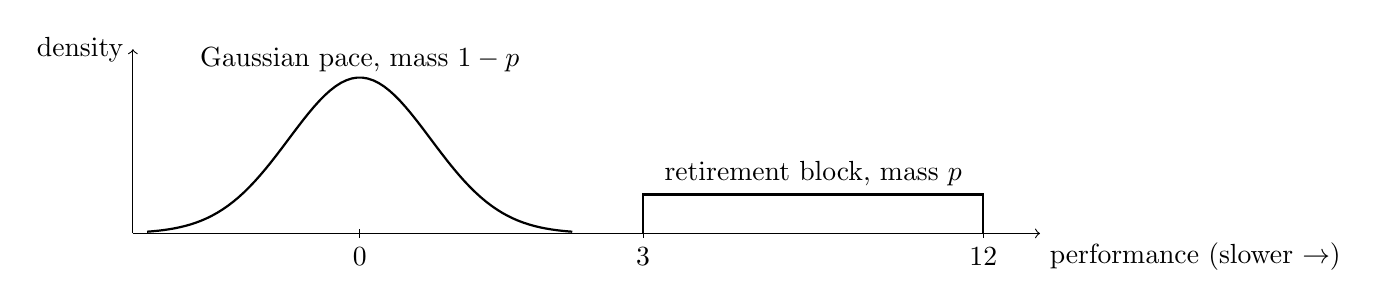
\begin{tikzpicture}[scale=0.9]
  \draw[->] (-3.2,0) -- (9.6,0) node[below right] {performance (slower $\rightarrow$)};
  \draw[->] (-3.2,0) -- (-3.2,2.6) node[left] {density};
  \draw[thick,domain=-3:3,samples=80] plot (\x,{2.2*exp(-0.5*\x*\x)});
  \node at (0,2.45) {Gaussian pace, mass $1-p$};
  \draw[thick] (4,0) -- (4,0.55) -- (8.8,0.55) -- (8.8,0);
  \node at (6.4,0.85) {retirement block, mass $p$};
  \draw (0,0.06) -- (0,-0.06) node[below] {$0$};
  \draw (4,0.06) -- (4,-0.06) node[below] {$3$};
  \draw (8.8,0.06) -- (8.8,-0.06) node[below] {$12$};
\end{tikzpicture}
\caption{The two-component base density: a continuous Gaussian pace
component and a separated rectangular block of slow mass representing
retirement.}
\label{fig:slab}
\end{figure}

We compare this density against the Gaussian default and against generic
departures from normality: symmetric heavy tails, skew, and a
concentrated pace core. All configurations differ only in the base
density.

\begin{center}
\begin{tabular}{lccc}
\toprule
base density & log loss & ECE & rank-PIT \\
\midrule
era-adaptive block & \textbf{2.200} & .016 & .185 \\
$N(0,1)$ plus 25\% block & 2.203 & .015 & .158 \\
skew-normal ($a{=}2$) & 2.222 & \textbf{.010} & .165 \\
Gaussian & 2.225 & .015 & .176 \\
tight core (0.5) plus 25\% block & 2.254 & .013 & \textbf{.136} \\
Student-$t$ ($\nu{=}5$) & 2.271 & .018 & .171 \\
near-Dirac core plus block & 2.42--2.52 & --- & --- \\
\bottomrule
\end{tabular}
\end{center}

The block improves every metric relative to the Gaussian. Because a fixed
25\% mass is wrong for most decades of the table in Section 1, the
era-adaptive variant estimates $p$ from a trailing window of observed
retirement frequency, using past races only. It attains the best log loss
and rank correlation of any configuration tested, and its fitted mass
declines across the dataset to finish near the modern retirement rate.

The generic departures fail, which sharpens the conclusion. Symmetric
heavy tails hurt increasingly as tails fatten, because symmetry places
equal mass on implausibly fast performances. Skew-normal noise changes
little, consistent with two facts about rank data: the difference of two
independent identically distributed noises is symmetric whatever their
skew, and ranks are invariant to monotone transformations of the time
scale. A near-Dirac pace core loses about 0.2 of log loss, showing that
variation from strategy, traffic and weather is comparable in size to
ability differences. The value is not in non-normality as such. It is in
matching the actual structure of the noise, here a separated mixture
component with a physical meaning, and only a system with a free noise
density can express that.

\section{Comparison with betting odds}

As a secondary exercise we compare the ratings with bookmaker prices. No
public archive of Formula 1 winner odds exists; from Wayback Machine
captures of odds-comparison pages we recovered full-field consensus
probabilities for 144 races between 2008 and 2025 (medians across roughly
twenty bookmakers, normalized to remove the margin). Snapshot timing
matters: a price taken after qualifying incorporates the grid and is not a
baseline for any forecast made without it. We therefore stratify the 135
covered post-warm-up races by snapshot date and match information tiers,
comparing pre-qualifying prices against results-only ratings and race-day
prices against ratings that observe each grid as an additional ranking
event before predicting.

\begin{center}
\begin{tabular}{lcccc}
\toprule
stratum & races & market & tier-matched ratings & gap (se) \\
\midrule
pre-qualifying & 88 & 1.581 & 2.177 & +0.60 (.08) \\
qualifying day & 26 & 1.622 & 1.820 & +0.20 (.11) \\
race day & 21 & 1.310 & 1.625 & +0.31 (.14) \\
\bottomrule
\end{tabular}
\end{center}

The stratification shows the market's advantage is mostly not the grid:
the full gap is already present in pre-qualifying prices, which reflect
current car performance, testing and practice pace. Grid information
matters (observing the grid improves the ratings from 2.177 to 1.926 on
the pre-qualifying stratum) but does not close the gap, and remarkably the
pre-qualifying market outperforms even ratings holding the realized grid,
information those prices could not contain. Pooling tests confirm the
point: on the pre-qualifying stratum every rating system considered in
Section 3, including the grid-aware variant, receives a fitted weight of
zero alongside the market price, and the fitted market temperature does
not validate out of sample at this sample size. Within the limits of the
record, Formula 1 winner markets appear efficient with respect to
results-based ratings at every information tier we can construct.

\section{Limitations}

Constructor effects are folded into driver ratings; separating driver from
car is the natural next study. Retirements enter tied at the back, which
discards the official ordering of retirees by laps completed. The ratings
are one-dimensional, with no axis for wet weather or circuit type. The
odds record is as described in Section 5, and in particular the grid
position asymmetry means the market comparison understates what a
qualifying-aware rating could achieve.

\section*{Reproducibility}

Each table is one command from the \texttt{winning} package
(\texttt{github.com/microprediction/winning}):
\texttt{python -m winning.benchmarks.run\_benchmark --dataset f1} for
Section 3, and the scripts \texttt{research/f1\_dirac\_disaster.py},
\texttt{research/t\_sweep.py}, \texttt{research/f1\_era\_slab.py},
\texttt{research/f1\_odds\_fetch.py}, \texttt{research/f1\_odds\_parse.py}
and \texttt{research/f1\_market\_test.py} for Sections 4 and 5. Race data
is fetched at run time from f1db (CC-BY-4.0). The lattice machinery is the
\texttt{thurstone} package; the underlying ability transform is described
in Cotton, \emph{SIAM J.\ Financial Mathematics} 12(1), 2021.

\end{document}
